% !TEX root = ../entropy.tex

\section{Additional results}%
\label{sec:additional_results}

\subsection{Endogeneity}%
\label{sub:endogeneity}

As discussed in Section~\ref{sub:estimation}, one concern one might have about
our results in Section~\ref{sec:results} is reverse causality:
transferring money into savings accounts might change the distribution of spend
categories and thus change entropy. As noted previously, this is not a major
concern because of the way we calculate savings and spend profiles: savings are
calculated as the sum of inflows into savings accounts, while spend profiles
are based on the classification of spend transactions in current accounts, and
transfers from current to savings accounts are labelled as such and not treated
as spend transactions.

However, because transaction labelling is imperfect, it is possible that some
transfers are misclassified as spends and included in the calculation of
entropy scores. One way to deal with this is to lag entropy scores by one
period. Table~\ref{tab:reg_has_inflows_lag} presents results similar to the main
results in the main text, but using entropy lagged by one year-month period as
the independent variable of interest. We can see that the results are very
similar to thos presented above.

\def\yvars{has_inflows}
\foreach \y in \yvars {
    \input{\tabdir/reg_\y_lag.tex}
}


\subsection{Further results by financial resilience}%
\label{sub:results_by_financial_resilience}

The Tables below show results presented in
Section~\ref{sub:effect_of_financial_resilience} for alternative entropy
variables. 

\def\evars{entropy_tag, entropy_merchant}
\foreach \e in \evars {
    \input{\tabdir/reg_has_inflows_\e_z_inc_quint.tex}
    \input{\tabdir/reg_has_inflows_\e_sz_inc_quint.tex}
    \input{\tabdir/reg_has_inflows_\e_z_inc_var_quint.tex}
    \input{\tabdir/reg_has_inflows_\e_sz_inc_var_quint.tex}
}

% \subsection{Old stuff}%
% \label{sub:old_stuff}
% \newpage
% \subsection{Exploration}%
% \label{sub:exploration}
% 
\begin{table}[htbp]
   \centering
   \tiny
   \begin{threeparttable}[b]
      \caption{\label{tab:reg_has_sa_inflows_explore} Entropy exploration}
      \begin{tabular}{lcccccc}
         \tabularnewline \midrule \midrule
         Dependent Variable: & \multicolumn{6}{c}{Has savings}\\
         Model:                    & (1)             & (2)              & (3)             & (4)             & (5)             & (6)\\  
         \midrule
         \emph{Variables}\\
         Entropy (48 cats)         & 0.031$^{***}$   & 0.057$^{***}$    & 0.031$^{***}$   & 0.006           & 0.040$^{***}$   & 0.049$^{***}$\\   
                                   & [0.020; 0.042]  & [0.044; 0.070]   & [0.021; 0.042]  & [-0.008; 0.021] & [0.029; 0.052]  & [0.023; 0.074]\\   
         Entropy (48 cats, smooth) &                 & -0.034$^{***}$   &                 &                 &                 & -0.027$^{***}$\\   
                                   &                 & [-0.043; -0.026] &                 &                 &                 & [-0.046; -0.008]\\   
         Spend txns                &                 &                  & 0.001$^{***}$   &                 &                 & 0.001$^{**}$\\   
                                   &                 &                  & [0.001; 0.001]  &                 &                 & [0.000; 0.001]\\   
         Unique categories         &                 &                  &                 & 0.006$^{***}$   &                 & -0.001\\   
                                   &                 &                  &                 & [0.004; 0.008]  &                 & [-0.004; 0.002]\\   
         Category count variation  &                 &                  &                 &                 & 0.000$^{***}$   & -0.000$^{**}$\\   
                                   &                 &                  &                 &                 & [0.000; 0.000]  & [-0.000; -0.000]\\   
         Paid with credit (\%)     & 0.000           & -0.000           & -0.000          & -0.000          & -0.000          & -0.000\\   
                                   & [-0.000; 0.000] & [-0.001; 0.000]  & [-0.001; 0.000] & [-0.000; 0.000] & [-0.000; 0.000] & [-0.001; 0.000]\\   
         Month spend               & 0.010$^{***}$   & 0.006$^{***}$    & 0.005$^{***}$   & 0.008$^{***}$   & 0.008$^{***}$   & 0.005$^{***}$\\   
                                   & [0.007; 0.012]  & [0.003; 0.008]   & [0.003; 0.008]  & [0.005; 0.010]  & [0.005; 0.010]  & [0.003; 0.008]\\   
         Urban                     & -0.024          & -0.019           & -0.019          & -0.024          & -0.022          & -0.018\\   
                                   & [-0.235; 0.187] & [-0.233; 0.196]  & [-0.230; 0.192] & [-0.234; 0.187] & [-0.235; 0.190] & [-0.230; 0.195]\\   
         Month income              & 0.002           & 0.000            & -0.000          & 0.001           & 0.001           & -0.000\\   
                                   & [-0.005; 0.009] & [-0.007; 0.007]  & [-0.007; 0.006] & [-0.005; 0.008] & [-0.006; 0.008] & [-0.007; 0.007]\\   
         Has income in month       & 0.044$^{***}$   & 0.035$^{**}$     & 0.038$^{**}$    & 0.040$^{***}$   & 0.041$^{***}$   & 0.035$^{**}$\\   
                                   & [0.014; 0.074]  & [0.005; 0.065]   & [0.008; 0.068]  & [0.010; 0.070]  & [0.011; 0.071]  & [0.006; 0.065]\\   
         Income variability        & -0.003          & -0.003           & -0.003          & -0.003          & -0.003          & -0.003\\   
                                   & [-0.012; 0.006] & [-0.012; 0.006]  & [-0.012; 0.005] & [-0.012; 0.006] & [-0.012; 0.006] & [-0.012; 0.005]\\   
         Rent payment              & 0.024$^{**}$    & 0.023$^{**}$     & 0.024$^{**}$    & 0.022$^{**}$    & 0.024$^{**}$    & 0.024$^{**}$\\   
                                   & [0.005; 0.044]  & [0.004; 0.043]   & [0.005; 0.043]  & [0.002; 0.041]  & [0.005; 0.043]  & [0.005; 0.043]\\   
         Mortgage payment          & 0.017           & 0.014            & 0.016           & 0.013           & 0.016           & 0.016\\   
                                   & [-0.007; 0.041] & [-0.009; 0.038]  & [-0.008; 0.040] & [-0.011; 0.037] & [-0.008; 0.040] & [-0.008; 0.040]\\   
         Loan repayment            & 0.005           & 0.003            & 0.004           & 0.001           & 0.004           & 0.003\\   
                                   & [-0.011; 0.020] & [-0.013; 0.018]  & [-0.012; 0.019] & [-0.014; 0.017] & [-0.011; 0.020] & [-0.012; 0.019]\\   
         Benefits                  & -0.007          & -0.011           & -0.011          & -0.009          & -0.009          & -0.011\\   
                                   & [-0.045; 0.031] & [-0.049; 0.027]  & [-0.048; 0.027] & [-0.047; 0.029] & [-0.047; 0.029] & [-0.049; 0.027]\\   
         \midrule
         \emph{Fixed-effects}\\
         User id                   & Yes             & Yes              & Yes             & Yes             & Yes             & Yes\\  
         Calendar month            & Yes             & Yes              & Yes             & Yes             & Yes             & Yes\\  
         \midrule
         \emph{Fit statistics}\\
         Observations              & 83,935          & 83,935           & 83,935          & 83,935          & 83,935          & 83,935\\  
         R$^2$                     & 0.42841         & 0.42940          & 0.42929         & 0.42879         & 0.42877         & 0.42950\\  
         Within R$^2$              & 0.00341         & 0.00512          & 0.00494         & 0.00406         & 0.00403         & 0.00530\\  
         \midrule \midrule
         \multicolumn{7}{l}{\emph{Clustered (User id) co-variance matrix, 95\% confidence intervals in brackets}}\\
         \multicolumn{7}{l}{\emph{Signif. Codes: ***: 0.01, **: 0.05, *: 0.1}}\\
      \end{tabular}
      
      \begin{tablenotes}\footnotesize
         \item Notes: Spend and income variables are in \pounds'000.
      \end{tablenotes}
   \end{threeparttable}
\end{table}



% 
\begin{table}[htbp]
   \centering
   \tiny
   \begin{threeparttable}[b]
      \caption{\label{tab:reg_has_sa_inflows_explore} Entropy exploration}
      \begin{tabular}{lccccc}
         \tabularnewline \midrule \midrule
         Dependent Variable: & \multicolumn{5}{c}{Entropy (48 cats)}\\
         Model:                    & (1)            & (2)            & (3)            & (4)              & (5)\\  
         \midrule
         \emph{Variables}\\
         Entropy (48 cats, smooth) & 0.274$^{***}$  &                &                &                  & 0.539$^{***}$\\   
                                   & [0.264; 0.285] &                &                &                  & [0.528; 0.550]\\   
         Spend txns                &                & 0.001$^{***}$  &                &                  & 0.010$^{***}$\\   
                                   &                & [0.001; 0.002] &                &                  & [0.010; 0.010]\\   
         Unique categories         &                &                & 0.097$^{***}$  &                  & 0.081$^{***}$\\   
                                   &                &                & [0.096; 0.099] &                  & [0.079; 0.082]\\   
         Category count variation  &                &                &                & -0.000$^{***}$   & -0.000$^{***}$\\   
                                   &                &                &                & [-0.000; -0.000] & [-0.000; -0.000]\\   
         \midrule
         \emph{Fixed-effects}\\
         User id                   & Yes            & Yes            & Yes            & Yes              & Yes\\  
         Calendar month            & Yes            & Yes            & Yes            & Yes              & Yes\\  
         \midrule
         \emph{Fit statistics}\\
         Observations              & 83,935         & 83,935         & 83,935         & 83,935           & 83,935\\  
         R$^2$                     & 0.66423        & 0.59311        & 0.77939        & 0.61808          & 0.92879\\  
         Within R$^2$              & 0.17916        & 0.00530        & 0.46067        & 0.06634          & 0.82592\\  
         \midrule \midrule
         \multicolumn{6}{l}{\emph{Clustered (User id) co-variance matrix, 95\% confidence intervals in brackets}}\\
         \multicolumn{6}{l}{\emph{Signif. Codes: ***: 0.01, **: 0.05, *: 0.1}}\\
      \end{tabular}
      
      \begin{tablenotes}\footnotesize
         \item Notes: Spend and income variables are in \pounds'000.
      \end{tablenotes}
   \end{threeparttable}
\end{table}



% 
\begin{table}[htbp]
   \centering
   \tiny
   \begin{threeparttable}[b]
      \caption{\label{tab:reg_has_sa_inflows_explore} Entropy exploration}
      \begin{tabular}{lccccc}
         \tabularnewline \midrule \midrule
         Dependent Variable: & \multicolumn{5}{c}{Entropy (48 cats)}\\
         Model:                    & (1)            & (2)            & (3)              & (4)              & (5)\\  
         \midrule
         \emph{Variables}\\
         Entropy (48 cats, smooth) & 0.212$^{***}$  &                &                  &                  & 0.530$^{***}$\\   
                                   & [0.208; 0.216] &                &                  &                  & [0.526; 0.533]\\   
         Spend txns                &                & 0.003$^{***}$  &                  &                  & 0.010$^{***}$\\   
                                   &                & [0.003; 0.003] &                  &                  & [0.010; 0.010]\\   
         Unique categories         &                &                & 0.098$^{***}$    &                  & 0.080$^{***}$\\   
                                   &                &                & [0.097; 0.098]   &                  & [0.080; 0.081]\\   
         Category count variation  &                &                &                  & -0.000$^{***}$   & -0.000$^{***}$\\   
                                   &                &                &                  & [-0.000; -0.000] & [-0.000; -0.000]\\   
         (Intercept)               & 0.501$^{***}$  & 0.213$^{***}$  & -1.079$^{***}$   & 0.508$^{***}$    & -1.228$^{***}$\\   
                                   & [0.497; 0.504] & [0.205; 0.221] & [-1.088; -1.069] & [0.503; 0.512]   & [-1.232; -1.223]\\   
         \midrule
         \emph{Fit statistics}\\
         Observations              & 83,935         & 83,935         & 83,935           & 83,935           & 83,935\\  
         R$^2$                     & 0.10447        & 0.04296        & 0.56104          & 0.02614          & 0.88513\\  
         Adjusted R$^2$            & 0.10446        & 0.04295        & 0.56104          & 0.02613          & 0.88513\\  
         \midrule \midrule
         \multicolumn{6}{l}{\emph{IID co-variance matrix, 95\% confidence intervals in brackets}}\\
         \multicolumn{6}{l}{\emph{Signif. Codes: ***: 0.01, **: 0.05, *: 0.1}}\\
      \end{tabular}
      
      \begin{tablenotes}\footnotesize
         \item Notes: Spend and income variables are in \pounds'000.
      \end{tablenotes}
   \end{threeparttable}
\end{table}



% % 
\begin{table}[htbp]
   \centering
   \tiny
   \begin{threeparttable}[b]
      \caption{\label{tab:reg_has_sa_inflows_explore} Entropy exploration}
      \begin{tabular}{lc}
         \tabularnewline \midrule \midrule
         Dependent Variable:       & Has savings\\  
         Model:                    & (1)\\  
         \midrule
         \emph{Variables}\\
         Entropy (48 cats, smooth) & -0.012$^{***}$\\   
                                   & [-0.016; -0.008]\\   
         (Intercept)               & 0.369$^{***}$\\   
                                   & [0.366; 0.373]\\   
         \midrule
         \emph{Fit statistics}\\
         Observations              & 83,935\\  
         R$^2$                     & 0.00040\\  
         Adjusted R$^2$            & 0.00039\\  
         \midrule \midrule
         \multicolumn{2}{l}{\emph{IID co-variance matrix, 95\% confidence intervals in brackets}}\\
         \multicolumn{2}{l}{\emph{Signif. Codes: ***: 0.01, **: 0.05, *: 0.1}}\\
      \end{tabular}
      
      \begin{tablenotes}\footnotesize
         \item Notes: Spend and income variables are in \pounds'000.
      \end{tablenotes}
   \end{threeparttable}
\end{table}




% \newpage
% \begin{figure}[H]
%     \caption{Diagnostics}
%     \label{fig:diagnostics}
%     \begin{center}
%         \includegraphics[width=0.9\textwidth]{\figdir/diagnostics.png}
%     \end{center}
% \end{figure}

% \newpage
% \begin{figure}[H]
%     \caption{Entropy and unique tags}
%     \label{fig:entropy_tag_vs_nunique}
%     \begin{center}
%         \includegraphics[width=0.9\textwidth]{\figdir/entropy_tag_vs_nunique.png}
%     \end{center}
% \end{figure}


\subsection{Entropy components}%
\label{sub:entropy_components}

\begin{figure}[h]
    \centering 
    \caption{Correlation of entropy with its components}
    \label{fig:entropy_components}
    \includegraphics[width=.32\textwidth]{\figdir/scatter_entropy_nunique_tag_spend.png}
    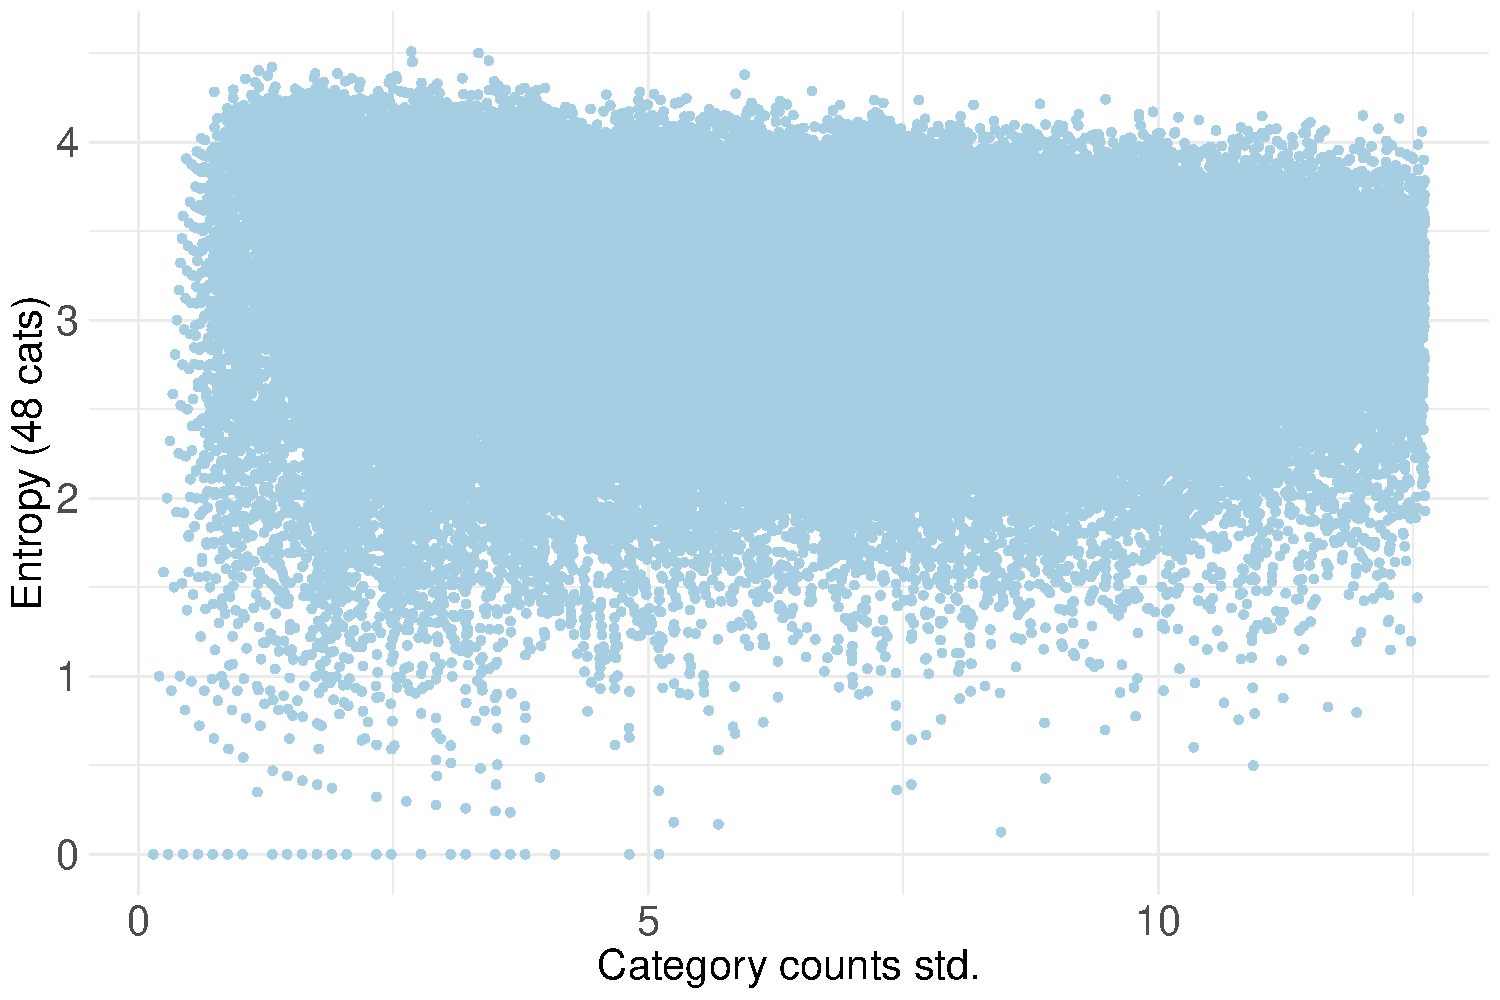
\includegraphics[width=.32\textwidth]{\figdir/scatter_entropy_std_tag_spend.png}
    \includegraphics[width=.32\textwidth]{\figdir/scatter_entropy_txns_count_spend.png}
    \fignote{\textwidth}{Correlation of 48-categories-based unsmoothed entropy
    with its three main components: the number of unique spending categories
with positive frequency counts (left), the standard deviation of those
frequency counts (middle), and the number of total spend transactions (left).}
\end{figure}

Figure~\ref{fig:entropy_components} shows the empirical relationship with our
48-categories-based unsmoothed entropy variable and these three
components.\footnote{To highlight the main features of the relationships we
have trimmed the component values at the 95th percentile.} We can see that for
the values we observe in the dataset, entropy increases monotonically in the
number of unique spending categories with positive frequency counts, has no
clear relationship with the standard deviation of those counts, and increases
in the number of total spending transactions up to about 175 transaction,
before being increasingly determined by other elements thereafter.


\subsection{Entropy correlations}%
\label{sub:entropy_correlations}



\begin{figure}[H]
    \centering 
    \caption{Effect of smoothing on entropy}
    \label{fig:scatter_facets}
    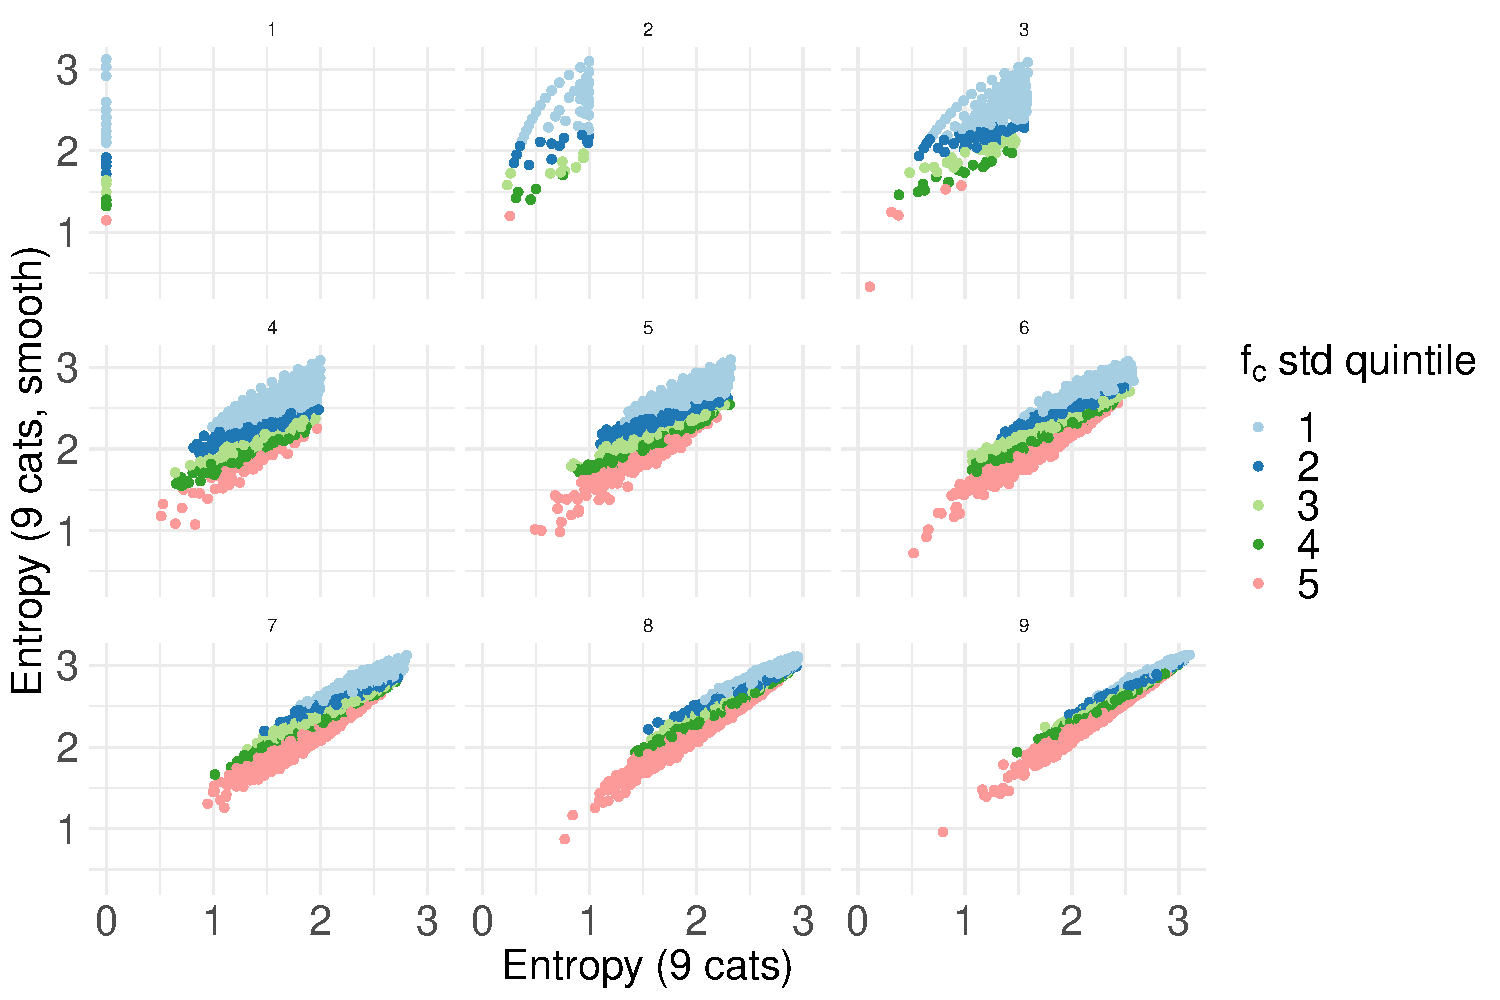
\includegraphics[width=\textwidth]{\figdir/scatter_facet_std_tag_q.png}
    % \fignote{\textwidth}{Effect of smoothing on entropy (top left) and entropy
    %     as a function of its three main components: the number of spending
    %     categories with positive frequency-counts (top right), the standard
    %     deviatioin of these counts (lower left), and the total number of
    % spending transaction (lower right). Value ranges for entropy components are
% trimmed at the 95th percentile.}
\end{figure}

\begin{figure}[H]
    \centering 
    \caption{Effect of smoothing on entropy}
    \label{fig:scatter_facets}
    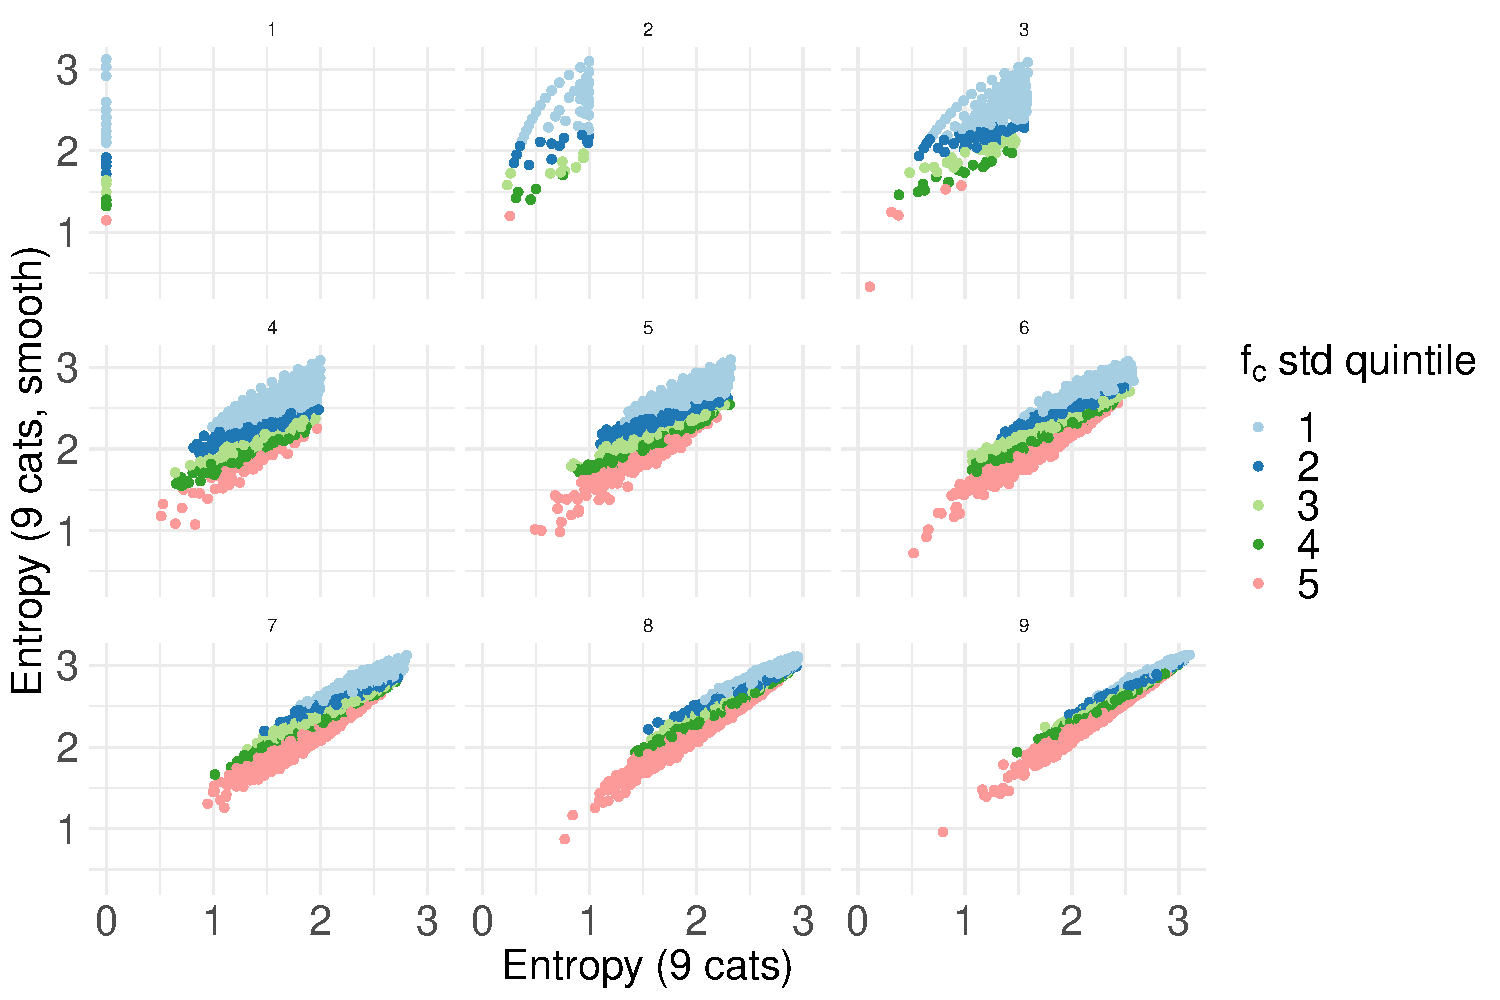
\includegraphics[width=\textwidth]{\figdir/scatter_facet_std_tag_q.png}
    % \fignote{\textwidth}{Effect of smoothing on entropy (top left) and entropy
    %     as a function of its three main components: the number of spending
    %     categories with positive frequency-counts (top right), the standard
    %     deviatioin of these counts (lower left), and the total number of
    % spending transaction (lower right). Value ranges for entropy components are
% trimmed at the 95th percentile.}
\end{figure}\newpage

